\section{An�lisis}\label{sec:discusion}

\subsection{}\label{subsec:analisis-1}

Las figuras~\ref{fig:d1},~\ref{fig:d2},~\ref{fig:d3},~\ref{fig:d4} y~\ref{fig:d5} representan las rectas $\tan{\alpha}$ frente a la intensidad $I$
para las distintas distancias $d$.


\begin{figure}[t!]
    \begin{center}
        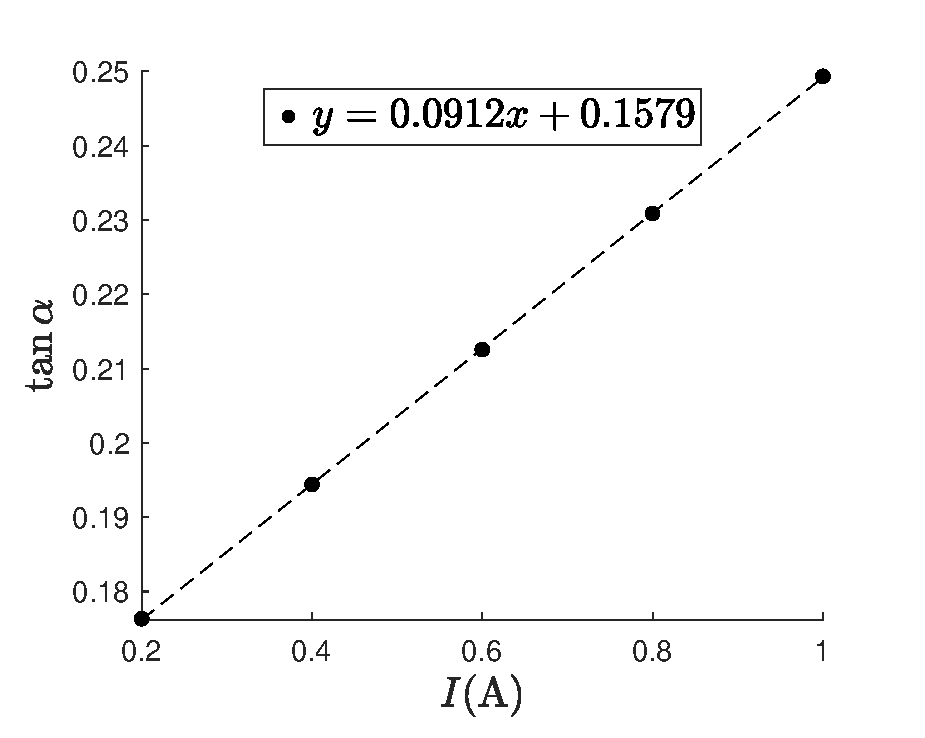
\includegraphics[width=0.8\columnwidth]{files/images/d1}
    \end{center}
    \caption{$\tan{\alpha}$ frente a $I$ para $d = 5\,$cm.}
    \label{fig:d1}
\end{figure}

\begin{figure}[t!]
    \begin{center}
        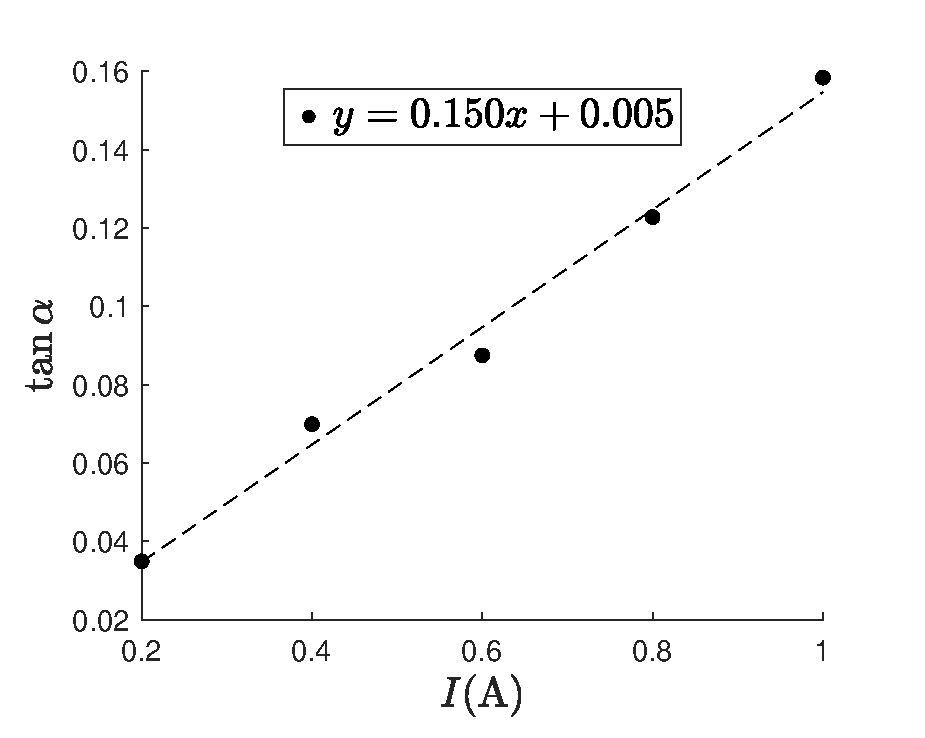
\includegraphics[width=0.8\columnwidth]{files/images/d2}
    \end{center}
    \caption{$\tan{\alpha}$ frente a $I$ para $d = 10\,$cm.}
    \label{fig:d2}
\end{figure}

\begin{figure}[t!]
    \begin{center}
        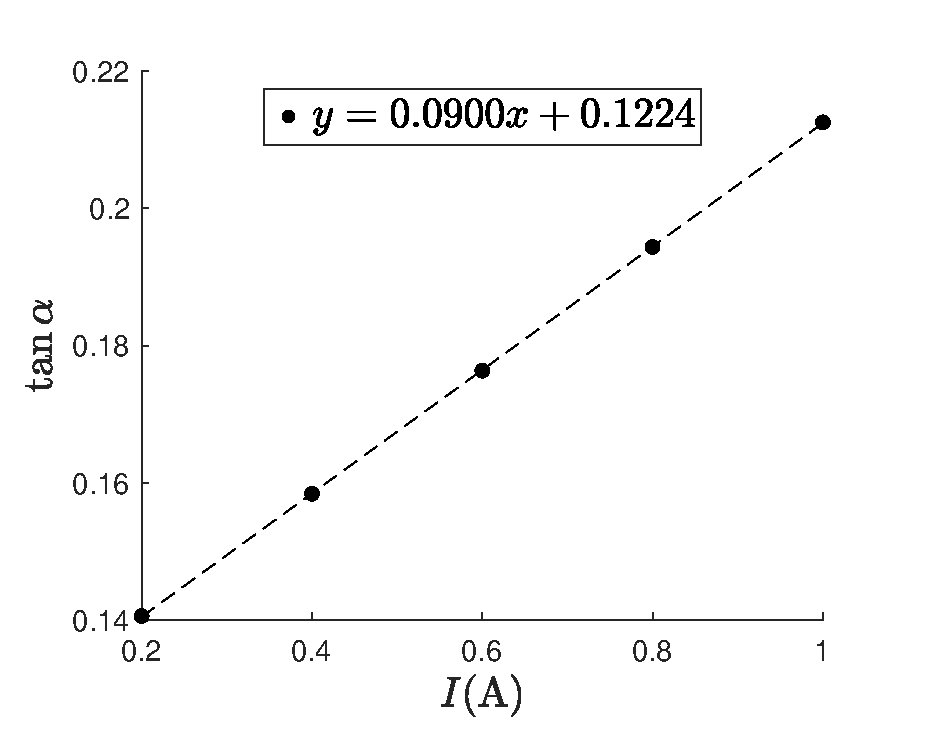
\includegraphics[width=0.8\columnwidth]{files/images/d3}
    \end{center}
    \caption{$\tan{\alpha}$ frente a $I$ para $d = 15\,$cm.}
    \label{fig:d3}
\end{figure}

\begin{figure}[t!]
    \begin{center}
        \includegraphics[width=0.8\columnwidth]{files/images/d4}
    \end{center}
    \caption{$\tan{\alpha}$ frente a $I$ para $d = 20\,$cm.}
    \label{fig:d4}
\end{figure}

\begin{figure}[t!]
    \begin{center}
        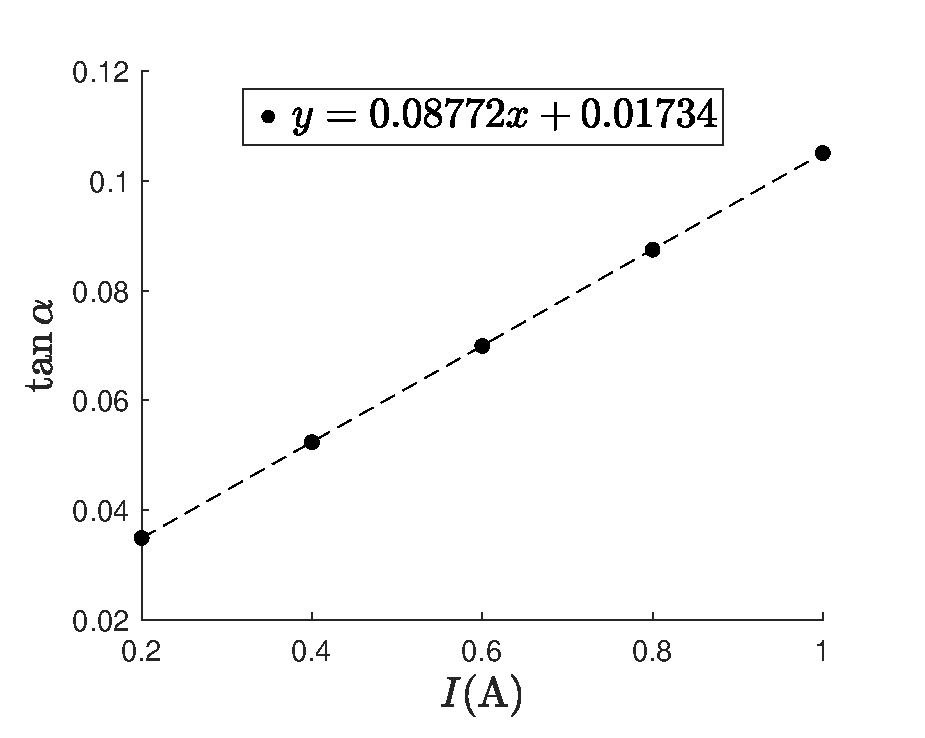
\includegraphics[width=0.8\columnwidth]{files/images/d5}
    \end{center}
    \caption{$\tan{\alpha}$ frente a $I$ para $d = 25\,$cm.}
    \label{fig:d5}
\end{figure}

\FloatBarrier

Seg�n la ecuaci�n~\ref{eq:tangente}, la pendiente de las rectas es:
\begin{equation*}
    a = \frac{\mu_0}{2\pi d H}
\end{equation*}

La tabla~\ref{tab:a} muestra los valores de la pendiente $a$ de las rectas para cada $d$.

\begin{table}[tbh]
    \center
    \caption{Rectas $\tan{\alpha}$ frente a $I$ con pendiente $a$ para diferentes distancias $d$.}
    \label{tab:a}
    \begin{centering}
        \begin{tabular}{|P{30px}|P{70px}|}
            \hline
            $d\,$(cm) & $a$                 \\
            \hline
            $0.05$    & $0.0912 \pm 0.0002$ \\
            $0.05$    & $0.0912 \pm 0.0002$ \\
            $0.05$    & $0.0912 \pm 0.0002$ \\
            $0.05$    & $0.0912 \pm 0.0002$ \\
            $0.05$    & $0.0912 \pm 0.0002$ \\
            \hline
        \end{tabular}
    \end{centering}
\end{table}

A partir de los valores de~\ref{tab:a}, obtenemos los distintos valores calculados de $H$, que se muestran en la tabla~\ref{tab:H}.

\begin{table}[tbh!]
    \center
    \caption{Componente horizontal del campo magn�tico terrestre $H$ calculado para distintas distancias $d$.}
    \label{tab:H}
    \begin{centering}
        \begin{tabular}{|P{30px}|P{70px}|}
            \hline
            $d\,$(cm) & $H$                 \\
            \hline
            $0.05$    & $0.0912 \pm 0.0002$ \\
            $0.05$    & $0.0912 \pm 0.0002$ \\
            $0.05$    & $0.0912 \pm 0.0002$ \\
            $0.05$    & $0.0912 \pm 0.0002$ \\
            $0.05$    & $0.0912 \pm 0.0002$ \\
            \hline
        \end{tabular}
    \end{centering}
\end{table}


El error en las medidas de $H$ se ha determinado mediante la expresi�n:
\begin{equation*}
    \epsilon_H = \frac{\mu_0}{2 \pi a d} \Bigl( \frac{\epsilon_d }{d} + \frac{\epsilon_a}{a}   \Bigr)
\end{equation*}